% -*- latex -*-
%-----------------------------------------------------------------------
%;  Copyright (C) 2017
%;  Associated Universities, Inc. Washington DC, USA.
%;
%;  This program is free software; you can redistribute it and/or
%;  modify it under the terms of the GNU General Public License as
%;  published by the Free Software Foundation; either version 2 of
%;  the License, or (at your option) any later version.
%;
%;  This program is distributed in the hope that it will be useful,
%;  but WITHOUT ANY WARRANTY; without even the implied warranty of
%;  MERCHANTABILITY or FITNESS FOR A PARTICULAR PURPOSE.  See the
%;  GNU General Public License for more details.
%;
%;  You should have received a copy of the GNU General Public
%;  License along with this program; if not, write to the Free
%;  Software Foundation, Inc., 675 Massachusetts Ave, Cambridge,
%;  MA 02139, USA.
%;
%;  Correspondence concerning AIPS should be addressed as follows:
%;          Internet email: aipsmail@nrao.edu.
%;          Postal address: AIPS Project Office
%;                          National Radio Astronomy Observatory
%;                          520 Edgemont Road
%;                          Charlottesville, VA 22903-2475 USA
%-----------------------------------------------------------------------
%Body of final AIPSletter for 31 December 2016

\documentclass[twoside]{article}
\usepackage{graphics}

\newcommand{\AIPRELEASE}{December 31, 2017}
\newcommand{\AIPVOLUME}{Volume XXXVII}
\newcommand{\AIPNUMBER}{Number 2}
\newcommand{\RELEASENAME}{{\tt 31DEC17}}
\newcommand{\OLDNAME}{{\tt 31DEC16}}
\newcommand{\NEWNAME}{{\tt 31DEC18}}
\newcommand{\Tsys}{${\rm T}_{\rm sys}$}

%macros and title page format for the \AIPS\ letter.
\input LET98.MAC

\newcommand{\MYSpace}{-11pt}

\normalstyle

\section{General developments in \AIPS}

\subsection{Reduction of VLB, VLA and ALMA data in \AIPS}

\AIPS\ continues to be the main software system for the reduction of
VLBI data from the VLBA and other telescopes.  Since 2010, there have
been numerous improvements to \AIPS\ that enable full calibration of
data from the Karl G. Jansky VLA and most imaging operations as well.
The one exception is the wide-band (bandwidth synthesis) deconvolution
algorithm (``MSMFS'') being developed in \CASA\ by Urvashi Rao
Venkata, for which there is no comparable function in \AIPS\@.
Calibrated $uv$ data may be exported from \AIPS\ in ``UVFITS'' format
for use in that program.  ALMA data may also be reduced in \AIPS,
although the package is not fully qualified to calibrate data from
linearly-polarized feeds.  See Appendix E of the \AIPS\ Cookbook,
available via the \AIPS\ web site, for details.

\subsection{\Aipsletter\ publication}

We have discontinued paper copies of the \Aipsletter\ other than for
libraries and NRAO staff.  The \Aipsletter\ will be available in
PostScript and pdf forms as always from the web site listed above and
will be shipped with all distributions of \AIPS\@.  It will be
announced on the bananas and MNJ list servers and, usually, in the
NRAO e-News mailing.

\subsection{Current and future releases}

We have formal \AIPS\ releases on an annual basis.  We recommend a
full binary installation method for both the frozen and development
versions for MacIntosh OS/X (Intel chips only), and Linux (32- and
64-bit) systems, but all architectures can do a full installation from
the source files.  There are also binary versions available for
\RELEASENAME\ for Solaris and Mac PPC chip architectures.  If you
develop \AIPS\ code locally {\it or have system managers that forbid
  the use of\/} {\tt rsync} or {\tt cvs}, you will need to do a
source-level installation.  The current release is called
\RELEASENAME\ and is now ``frozen.''  If you took a development copy
of this version at some earlier date, you should use the ``Midnight
Job'' (MNJ) to bring it up to date.  You need to run a MNJ only once
in 2018 to convert your copy of \RELEASENAME\ into the frozen version.
However, when patches to \RELEASENAME\ are announced in 2018, you may
apply them with the MNJ\@.  This \Aipsletter\ is intended to advise
you of corrections and improvements in this release.

We have begun a new version, called \NEWNAME, which is now under
development by the \AIPS\ Group.  You may fetch and install a complete
copy of this version at any time.  Having fetched \NEWNAME, you may
update your installation whenever you want by running the MNJ\@.  This
uses {\tt cvs}, {\tt rsync}, and/or transaction files to copy all
changed text files and then to copy the binary files or to compile the
code selectively based on the code changes and compilations we have
done.  We expect users to take their source-only or binary version of
\NEWNAME\ \AIPS\ over the Internet (via \emph{anonymous} ftp).  Both
versions require you to copy the installation procedure {\tt
  install.pl} via {\tt ftp}; the source-only version also requires you
to ftp the 135-Mbyte {\tt   \NEWNAME.tar.gz} compressed tar file.
Binary installations use only {\tt rsync}, while locally compiled
versions also use {\tt cvs}.  Linux sites will almost certainly have
{\tt cvs} installed; other sites may have installed it along with
other GNU tools.  Secondary MNJs will still be possible using {\tt
  ssh} or {\tt rcp} or NFS as with previous releases.  We have found
that {\tt cvs} works very well, although it has one quirk. If a site
modifies a file locally, but in an \AIPS-standard directory, {\tt cvs}
will detect the modification and attempt to reconcile the local
version with the NRAO-supplied version.  This usually produces a file
that will not compile or run as intended.  Use a new name for the task
or put a copy of the task and its help file in a private disk area
instead.

\AIPS\ is now copyright \copyright\ 1995 through 2017 by Associated
Universities, Inc., NRAO's parent corporation, but may be made freely
available under the terms of the Free Software Foundation's General
Public License (GPL)\@.  This means that User Agreements are no longer
required, that \AIPS\ may be obtained via anonymous ftp without
contacting NRAO, and that the software may be redistributed (and/or
modified), under certain conditions.  The full text of the GPL can be
found in the \texttt{15JUL95} \Aipsletter\ and is included with every
distribution in file {\tt \$AIPS\_ROOT/{\it release-name}/COPYING}\@.


\subsection{Installing a new version}

If compiling locally, new releases must be installed from the tar ball
for that release.  {\tt 31DEC15} and later versions contain
improvements to the code which should make local compilation more
reliable.  If using the binary installation, a full new installation
must also be done with {\tt rsync}.  When installing a new \AIPS\
release in a system that already has a previous release, we recommend
that {\tt install.pl} be used and that the previous release be left in
place, at least until the new installation has been verified.  If you
do this, then you will not have to re-edit the disk, printer, and tape
lists and can simply skip all those pages in the {\tt install.pl}
menus.  The old {\tt \$HOME/.AIPSRC} file may be left in place, but it
will need to be edited.  The lines giving the {\tt DOWNLOADED} and
{\tt UNPACKED} parameters should be cleared and the {\tt CCOMOPT} line
should be changed to point to the current release rather than the
previous one.  If you have made a special version of {\tt
  do\_daily.{\it host}}, you should preserve it under a new name and
restore it after the install. If you have an odd set of \AIPS\
versions, the {\tt \$AIPS\_ROOT/AIPSPATH.*SH} files may need to be
edited after the install to set the desired versions.  The file {\tt
  \$SYSLOCAL/UPDCONFIG} also needs to be edited to correct your e-mail
address(es).

{\tt 31DEC09} contains a change in the format of antenna files.
Previous releases will not understand the antenna coordinates for
arrays that were traditionally left-handed (VLBI primarily).  The
format change occurs automatically when any {\tt 31DEC09} or later
antenna-file specific code reads the file, after which older releases
will have difficulties.  {\tt 31DEC15} contains a change in the
headers of $uv$ data sets which will not be understood by previous
versions.  Note that the only version which we will patch for major
errors is \RELEASENAME; even \OLDNAME\ will no longer be changed.

%\section{Preview of coming attractions}

%The \NEWNAME\ release already contains a few changes that we decided
%were a bit risky or not needed in \RELEASENAME\@.

%\vfill\eject
\section{Improvements of interest to users in \RELEASENAME}

In the latter half of 2017, new tasks appeared including {\tt FGSPW}
to flag whole spectral windows on a scan, baseline, and polarization
basis when the scalar average amplitudes are excessive.  New tasks for
handling large pulse-cal tables include {\tt PCAVG} to average
pulse-cal tables over time, {\tt PCRMS} to flag a pulse-cal table
automatically based on various statistics, and {\tt PCHIS} to plot
histograms generated by {\tt PCRMS}\@.  The calibration of
linearly-polarized feeds has been partially addressed although there
is much room for improvement.  New tasks in the first half of 2017
include {\tt ELFIT} to fit polynomials to selected data from tables,
{\tt SYSOL} to calibrate Solar data sets using the SysPower table,
{\tt DFTIM} to make an image of visibility data at a celestial
coordinate as a function of time and frequency, {\tt AGAUS} to fit
Gaussians to absorption-line image cubes, {\tt ZAMAN} to fit Zeeman
splitting models to absorption line image cubes, and {\tt MODAB} to
prepare models for the Gaussian fitting tasks.

Normally, bugs which appear in an \AIPS\ {\tt TST} version and then
are fixed in that same version before its release get little or no
discussion in the \Aipsletter\@.  Since a rather large number of sites
now install the {\tt TST} version of \AIPS\ during its development,
this is somewhat of an oversight.  We urge you to run the ``Midnight
Job'' at least once after \RELEASENAME\ is frozen to bring it up to
date and to fix all bugs of this sort.  We urge active sites to use
the MNJ and, when something odd occurs, to examine {\tt CHANGE.DOC}
using the cgi tool available from the \AIPS\ documentation web page
({\tt http://www.aips.nrao.edu/aipsdoc.html}).  Please do not
hesitate to contact us via the NRAO help desk ({\tt
  https://help.nrao.edu}) or via e-mail {\tt daip@nrao.edu} with any
questions or suspicions that there are problems.

\subsection{VLBI matters}

\subsubsection{Pulse-cal tables}

The DiFX correlator is now capable of providing pulse-cal tones at
every MHz.  These complex data are written into text files archived in
full at the correlator site and may be written in the FITS-IDI output
files.  Since these data have very high signal-to-noise ratio, they
should be used wherever possible to assist with calibration.  During
the past 6 months, {\tt PCLOD} was changed to get the start date from
the data once rather than from the pulse-cal input and to offer the
option  of keeping or ignoring data outside of $uv$-data scans.  {\tt
  PCFLG} was changed to handle large input tables, to manage the sort
order carefully to avoid excessive sorting, to handle only times in
the specified time range, and to display times including day number
correctly even when there are no values in the current display.  {\tt
  PCAVG} is a new task to average pulse-cal tables over time.  {\tt
  PCFIT} was given a new option to suppress excessive jumps in delay
and the sign of the value written to the {\tt SN} table was switched.
{\tt PCPLT} was changed to honor {\tt XYRATIO} and {\tt ANTENNAS} and
to do horizontal axis labeling for any number of panels.  {\tt PCRMS}
is a new task intended to auto-edit pulse-cal tables.  This task looks
for individual channels that stick out too much from their neighbors
and for times where spectral windows deviate excessively from the
average and rms of that spectral window, polarization, and antenna.
{\tt PCRMS} does a surprisingly good job, but, if you want to examine
the data, {\tt PCRMS} has the option of writing a text file containing
the IF-average amplitude and its rms for every time in the table.  The
new task {\tt PCHIS} can read this file and plot histograms and
statistics.  The format of the file is rather general, so {\tt PCHIS}
may well have other uses.  The {\tt SN} table written by {\tt PCFIT}
has been shown to correct many, but not all, delay jumps found in real
data sets.


\subsubsection{Miscellaneous}

\begin{description}
\myitem{VLBAUTIL} was changed to update the URL for the EOP file.
\myitem{VLBARUN} was changed to avoid some {\tt BLEW TEMP C} failures.
\myitem{ANTAB} occasioned a change to allow 2560-character input lines
          in \AIPS' version of {\tt KEYIN} and a more extensive
          explanation of allowed input formats.
\myitem{APCAL} was given very much larger buffers to handle data sets
          with numerous spectral windows.
\myitem{KRING} was changed to write zeros rather than magic blanks for
          multi-band delay and dispersion when a polarization is
          flagged.  The calibration routines flagged all polarizations
          on the magic blanks.
\myitem{USUBA} was changed to allow more sources and entries up to the
          limits imposed by compilers.
\end{description}

\subsection{UV data: Miscellaneous}

Low-level routines in the calibration package were changed to allow
correct conversion of linear polarization data into full Stokes.  This
requires more widespread maintenance of the current parallactic
angle.  {\tt PCAL} still cannot handle a linear-polarization model but
works well on unpolarized calibrators at P-band.  The correction for
the X-Y phase difference is not available at this time, so full
calibration of linear polarization still does not work in \AIPS.

{\tt FGSPW} is a new task designed to find and flag spectral windows
that have been over-run by RFI\@.  It does a scalar-amplitude average
of all spectral channels in each scan and, for those baselines,
polarizations, and spectral windows that exceed a user-set cutoff,
flags the data in that scan.  It is a fast way to start the editing of
RFI-riddled data, before using {\tt SPFLG} or {\tt RFLAG}\@.

\begin{description}
\myitem{SY} table format changed and required some tasks to handle the
            tables differently and {\tt TYAPL} to change its internal
            version of the {\tt SY}-table flagging routine.
\myitem{Antenna} file opening and reformatting required changes to
            avoid leaving open files on errors, to specify enough
            keywords for data sets with 30 or more spectral windows,
            and to handle {\tt CASA}'s decision to honor only a
            portion of the new format.
\myitem{WIPER} was corrected to position displays properly on zoomed
            images.
\myitem{TVFLG} and similar tasks were corrected to handle time labels
            correctly including day number and to switch to fully
            blanked displays when no data are found for the selected
            image.  Label information became incorrect when the old,
            valid data remained on the display.  They were also
            changed to support {\tt STOKES = 'IQU'} and {\tt
              'IQUV'}\@.
\myitem{UVMOD} was changed to allow comment lines and negative flux
            components in the input text file.
\myitem{UVHOL} was corrected to handle unwanted data at the end of a
            print group and to allow a choice of whether the
            parallactic angle correction is applied or not on {\tt
              DOPOL > 0}.
\myitem{HOLOG} was changed to allow the option to compute the images
            from user-supplied parameters rather than the data and to
            simulate the effect of reference pointing.  It was changed
            to allow the specification of the frequency used to
            control the sampling and to request real and imaginary
            images rather than amplitude and phase.
\myitem{}
\end{description}

\subsection{Analysis: Miscellaneous}

\begin{description}
\myitem{RMFIT} was corrected to handle blotch drawing on
          pixel-replicated images when switching solutions between
          components and the units of the {\tt Q0} and {\tt U0} output
          images were corrected.  The option to display total
          polarization and polarization angle instead of Q and U was
          added.  Fitting is done in Q and U always.  The initial
          guess algorithm was substantially improved.
\myitem{FARS} was changed to write the one-dimensional RMTF (RM beam)
          as slice files, one each for real, imaginary, amplitude, and
          phase.
\myitem{FQUBE} was changed to use the {\tt FQ} planes in the current
          image and not to complain about {\tt FQ} values in the table
          which are not present in the image.  This allows {\tt SUBIM}
          to be used on an {\tt FQ} axis with the result being fed
          back into {\tt FQUBE}.
\myitem{TVSPC} acquired the options to label the images and to do a
          {\tt CURVALUE} display for any of the up to four displayed
          images and plots.
\end{description}

\subsection{Imaging and Display: Miscellaneous}

\begin{description}
\myitem{IMAGR} added {\tt OVRSWTCH}, {\tt FGAUSS}, and {\tt
        IMAGRPRM(11)} to the supported {\tt TELL} adverbs.
      Multi-scale Clean requires {\tt OVERLAP} $\ge 2$, so the code
      was changed to force this.
\myitem{RSPEC} was changed to use {\tt BLC} and {\tt TRC} in the
      normal way with {\tt DOINVER} controlling whether the statistics
      are done inside or outside the window.
\myitem{WETHR} was corrected to use the correct table-file format and
      to decide whether the {\tt TIME} column is double precision
      correctly.  An option to connect the plotted points was added.
\myitem{PCNTR} was changed to allow, with a warning, the drawing of
      polarization vectors on images lacking a proper celestial
      coordinate pair of axes.
\end{description}

\subsection{General}

Major difficulties arose over the last year or so with the {\tt LNX64}
binary version of \AIPS.  Beginning with Fedora 25, tasks started to
produce NaNs (``not-a-number'') in seemingly random but repeatable
places in the output.  {\tt IMAGR} was particularly affected, but
other tasks were as well.  Gradually other operating systems, more
modern than those used at NRAO, began to see the same problem.
Thinking that the very old version of the Intel compiler which we were
using might be at fault, we installed the latest Intel compiler
(version 18.0.0, dated 20170811).  All continued to work well on NRAO
computers, but the new version failed on those computers on which the
old versionhad failed.  The new failures occurred at even earlier
points than the NaNs.  Therefore, the binary version of \AIPS\ for
{\tt LNX64} is now computed with {\tt gfortran} and {\tt gcc} version
6.3.  This seems to work more or less everywhere.  During the test on
the latest Intel compiler, \AIPS\ code was corrected for
``over-stated'' {\tt EQUIVALENCE} statements and incorrect {\tt
  E}$w.d$ format codes.

\begin{description}
\myitem{ABORTASK} was given the {\tt NUMTELL} adverb to allow aborting
         tasks running under other {\tt POPS} numbers.
\myitem{WAITTASK} was given the {\tt NUMTELL} adverb to allow waiting
         on tasks running under other {\tt POPS} numbers.
\myitem{RUN} was corrected to avoid using magic text-file logical unit
         numbers so that verbs executed under nested {\tt RUN}s would
         have normal access to those LUNs.
\myitem{CookBook} was updated for changes noted above.
\end{description}

\section{Recent \AIPS\ Memoranda}

All \AIPS\ Memoranda are available from the \AIPS\ home page.  \AIPS\
Memo 117 was modified to describe the added columns in the {\tt SY} and
{\tt CD} tables for Solar data.  Memo 120 was modified for new
options in {\tt TVSPC}\@.  Memo 118 was modified for new options in
{\tt RMFIT}\@.  \AIPS\ Memo 123 was written to describe the usage of
the new, large pulse-cal tables in VLBI\@.

\begin{tabular}{lp{5.8in}}
{\bf 117} & {\bf \AIPS\ FITS File Format}\\
   &  Eric W. Greisen, NRAO\\
   &  June 19, 2017 (revised)\\
   &  \AIPS\ has been writing images and $uv$ data in FITS-format
   files for a very long time.  While these files have been used
   widely in the community, there is a perception that a detailed
   document in still required.  This memo is an attempt to meet that
   perception. \AIPS\ FITS files for $uv$ are conventions layered upon
   the standard FITS format to assist in the interchange of data
   recorded by interferometric telescopes, particularly by radio
   telescopes such as the EVLA and VLBA\@.
\end{tabular}

\begin{tabular}{lp{5.8in}}
{\bf 118} & {\bf Modeling Spectral Cubes in \AIPS}\\
   &  Eric W. Greisen, NRAO\\
   &  November 20, 2017 (revised)\\
   &    \AIPS\ has done Gaussian fitting along the $x$-axis of image cubes
  with task {\tt XGAUS} since the 1980s.  That task has recently been
  overhauled to be much easier to use and much more capable.  In like
  fashion, new tasks {\tt ZEMAN} and {\tt RMFIT} have been developed.
  The former fits the standard leakage and scaling terms for Stokes V
  cubes, including a new option to do this for each of the Gaussians
  found by {\tt XGAUS}\@.  The latter fits polarization models to
  Stokes Q and U cubes, using the output of Faraday Rotation Measure
  Synthesis (\AIPS\ task {\tt FARS}) to assist with initial guesses.
  The models can contain multiple components each with a polarization
  flux, angle, rotation measure, and rotation measure ``thickness.''
  The present memo will describe the functions of these tasks in some
  detail with numerous graphical examples.  A revision of this memo
  discusses changes made for the {\tt 31DEC15} release and two new
  tasks to plot spectra with model fits and a number of tasks which
  make visibility and image model files.  The November 2017
    revision includes new display options in {\tt RMFIT}\@.

\end{tabular}

\begin{tabular}{lp{5.8in}}
{\bf 120} & {\bf Exploring Image Cubes in \AIPS}\\
   &  Eric W. Greisen, NRAO\\
   &  July 22, 2017 (revised)\\
   &  \AIPS\ has recently acquired powerful tasks to fit models to the
  spectral axis of image cubes.  These tasks are easier to run if the
  user is already familiar with the general structure of the data
  cube.  A new task {\tt TVSPC} has been written to assist in
  acquiring this familiarity.  This task provides an exploration tool
  within the \AIPS\ environment, rather than requiring users to export
  their cubes to one or more of the many excellent visualization tools
  now available.  In the {\tt 31DEC17} version an additional data
  cube may be displayed one plane at a time.
\end{tabular}

\begin{tabular}{lp{5.8in}}
{\bf 123} & {\bf New Pulse-cal Capabilities for VLBI in \AIPS}\\
   &  Eric W. Greisen, NRAO\\
   &  October 30, 2017\\
   &  The DiFX correlator has acquired the capability of measuring and
   recording large numbers of pulse-cal tones, typically at intervals
   of 1 MHz through each spectral window.  These pulse-cal tones have
   very high signal-to-noise, but show a roll-off at the edges of each
   spectral window and usually have one or more single channels which
   have amplitude and residual phase differing significantly from the
   average for the spectral window.  \AIPS\ has acquired the ability
   to deal with these data including new tasks to display and edit
   them and to derive calibration from them.
\end{tabular}

\section{\AIPS\ Distribution}

From the NRAO system logs, we count apparent MNJ accesses, downloads
of the tar balls, and {\tt rsync} accesses by unique IP address.
Since DSL and some university and other connections may be assigned
different IP addresses at different times, this will be a bit of an
over-estimate of actual sites.  However, a single IP address is often
used to provide \AIPS\ to a number of computers, so these numbers are
at the same time an under-estimate of the number of computers running
current versions of \AIPS\@.  In 2017, a total of 408 different IP
addresses downloaded the frozen form of \OLDNAME\ and 874 IP
addresses downloaded \RELEASENAME\ in tarball or binary form.  Fully
644 IP addresses accessed the NRAO cvs master.  Each of these has at
least installed some version of \AIPS, but with the change to the MNJ
we are unable even to guess how many sites have run the MNJ\@.  The
total number of unique IP addresses in these three lists was 1383.
The table below shows these numbers as a function of year since we
began recording them.  The usual plot of numbers versus time, which we
omit, shows that 2016 and 2017 were very similar.
%\vfill
%\centerline{\resizebox{!}{3.7in}{\includegraphics{FIG/TWOPLOT.eps}}}

\begin{center}
\begin{tabular}{|rrrrrrrrr|}
\hline
 & & & & & {\tt TST} & {\tt NEW} & & Total \\
\noalign{\vspace{-1mm}}
year & {\tt TST} name & {\tt NEW} name & \hspace{1em}{\tt TST} &
 \hspace{1em}{\tt NEW} & binary & binary &
 \hspace{1em}{\tt cvs} & unique \\
\hline
2004 & {\tt 31DEC04} & {\tt 31DEC03} &  808 & 196 &      &     &  797
 & 1276 \\
2005 & {\tt 31DEC05} & {\tt 31DEC04} &  832 & 246 &  299 &  48 &  982
 & 1460 \\
2006 & {\tt 31DEC06} & {\tt 31DEC05} &  806 & 191 &  402 &  94 & 1050
 & 1398 \\
2007 & {\tt 31DEC07} & {\tt 31DEC06} &  965 & 277 &  669 & 161 & 1385
 & 1811 \\
2008 & {\tt 31DEC08} & {\tt 31DEC07} & 1058 & 246 &  986 & 303 & 1667
 & 2107 \\
2009 & {\tt 31DEC09} & {\tt 31DEC08} & 1228 & 307 & 1082 & 478 & 1855
 & 2399 \\
2010 & {\tt 31DEC10} & {\tt 31DEC09} & 1228 & 307 & 1203 & 477 & 1914
 & 2416 \\
2011 & {\tt 31DEC11} & {\tt 31DEC10} & 1105 & 270 & 1064 & 424 & 1747
 & 2228 \\
2012 & {\tt 31DEC12} & {\tt 31DEC11} &  940 & 284 & 1028 & 396 & 1309
 & 1698 \\
2013 & {\tt 31DEC13} & {\tt 31DEC12} & 1014 & 307 &  990 & 443 & 1264
 & 1937 \\
2014 & {\tt 31DEC14} & {\tt 31DEC13} & 1045 & 333 &  848 & 431 & 1023
 & 1843 \\
2015 & {\tt 31DEC15} & {\tt 31DEC14} & 1104 & 309 & 1001 & 350 & 1070
 & 1817 \\
2016 & {\tt 31DEC16} & {\tt 31DEC15} &  878 & 222 &  788 & 372 &  761
 & 1330 \\
2017 & {\tt 31DEC17} & {\tt 31DEC16} &  874 & 408 &  768 & 386 &  644
 & 1383 \\
\hline
\end{tabular}
\end{center}
\vfill\eject

\section{Patch Distribution for \OLDNAME}

Because of the extensive use of binary installations, we now patch the
master copy of the most recently frozen version.  Older versions are
not corrected even for egregious errors.  Thus, \OLDNAME\ was patched
during 2017 and \RELEASENAME\ will be patched as needed during 2018.
Your copy of them may be corrected simply by running a Midnight Job.
Information about patches and the code may be found using links from
the main \AIPS\ web page or by  {\it anonymous} \ftp\ to the NRAO
server {\tt ftp.aoc.nrao.edu}.  Documentation about patches to a
release is placed on this site at {\tt pub/software/aips/}{\it
  release-name} and the code is placed in suitable sub-directories
below this.  Patches to older releases are kept here as well, but they
will require local compilation.

The \OLDNAME\ release is no longer available for installation and will
no longer receive patches even for egregious errors.  It had a number
of important patches during 2017.  They are
\begin{enumerate}
  \item\ {\tt POSSM} would not label correlation functions in seconds
    {\it 2017-01-04.}
  \item\ {\tt ATLOD} would not open disk files properly. {\it
      2017-01-06.}
  \item\ {\tt CCRES} did not honor blanked pixels. {\it 2017-01-12.}
  \item\ {\tt DFTPL} did not use the correct frequencies when {\tt BIF
      > 1}. {\it 2017-01-31.}
  \item\ {\tt DBCON} scaled uvw wrongly when combining data sets of
    different frequencies. {\it 2017-02-24.}
  \item\ {\tt DFTPL} did not address data correctly when the input had
    more than one Stokes. {\it 2017-02-28.}
  \item\ {\tt BPASS} did not normalize linear polarization  bandpasses
    correctly for normalization type 1. {\it 2017-03-08.}
  \item\ Automatic spectral index determination from the {\tt SU}
    table had problems when one or more IFs had no flux value. {\it
      2017-03-21.}
  \item\ {\tt UVMOD} did not handle frequencies correctly with
    spectral index {\it 2017-03-21.}
  \item\ {\tt SPIXR} did not label the output images with the
    frequency for which they were determined (1 GHz). {\it 2017-03-31.}
  \item\ {\tt PCAL} miscomputed the flux at 1 GHz for known sources at
    low frequency {\it 2017-06-06.}
  \item\ {\tt SQASH} mishandled {\tt BLC, TRC}  {\it 2017-06-21.}
  \item\ {\tt UVLSF} copied tables twice to the output continuum data
    set. {\it 2017-06-30.}
  \item\ {\tt SCMAP} and {\tt SCIMG} messed up the self-cal step when
    the number of IFs was not the same as the number of polarizations.
    {\it 2017-07-03.}
  \item\ {\tt PCAL} left a file open when an IF had no data in
    spectral mode, causing failure on the next IF. {\it 2017-07-11.}
\end{enumerate}
\vfill\eject

% Order form and mailer page
%\cleardoublepage
\pagestyle{empty}
%\vfill
%\centerline{\resizebox{!}{23.3cm}{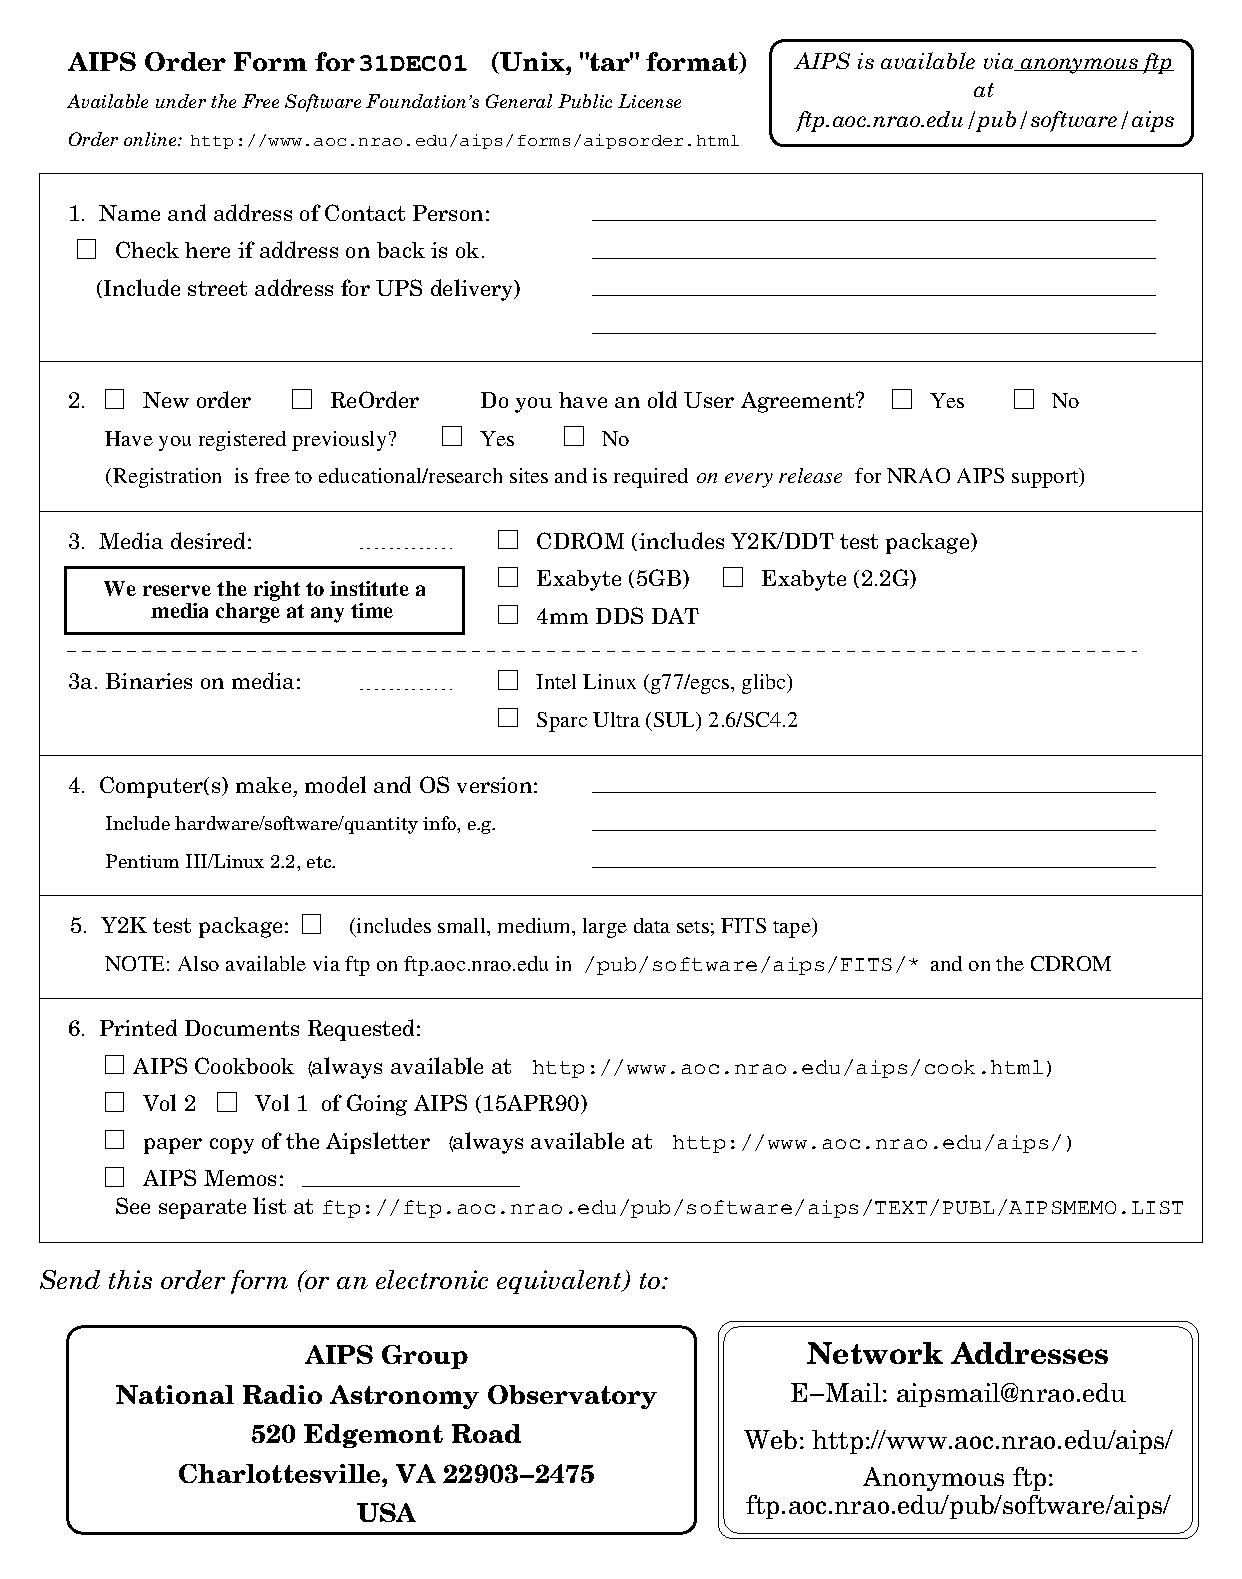
\includegraphics{FIG/AIPSORDER.PS}}}
\vfill\eject
\vbox to 4.4in{
\vspace{12pt}
%\centerline{\rotatebox{-90}{\resizebox{!}{3.5in}{%
%\includegraphics{FIG/Mandrill.color.plt}}}}
\centerline{\resizebox{!}{3.5in}{\includegraphics{FIG/Mandrill.eps}}}
\vspace{12pt}
\centerline{{\huge \tt \AIPRELEASE}}
\vspace{12pt}
\vfill}
\phantom{...}
\centerline{\resizebox{!}{!}{\includegraphics{FIG/AIPSLETS.PS}}}

\end{document}

